% This file was created by matlab2tikz.
%
%The latest updates can be retrieved from
%  http://www.mathworks.com/matlabcentral/fileexchange/22022-matlab2tikz-matlab2tikz
%where you can also make suggestions and rate matlab2tikz.
%
\definecolor{mycolor1}{rgb}{0.00000,0.44700,0.74100}%
\definecolor{mycolor2}{rgb}{0.85000,0.32500,0.09800}%
%
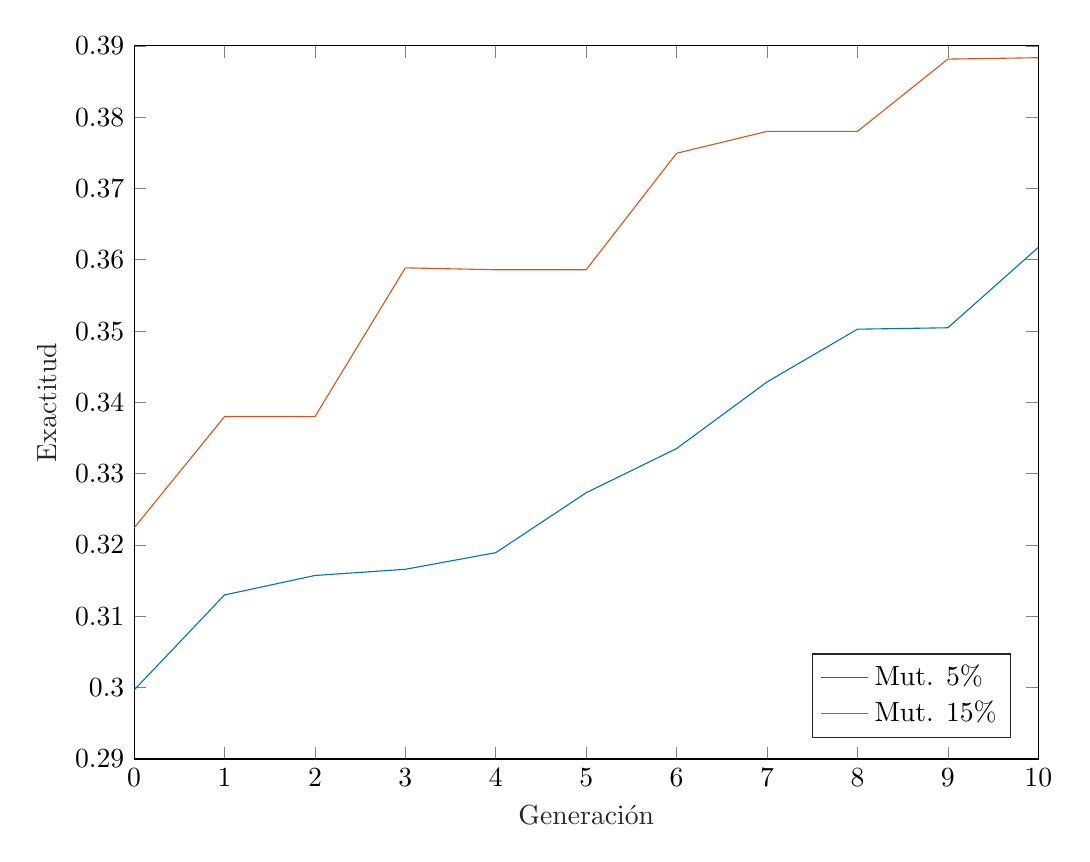
\begin{tikzpicture}

\begin{axis}[%
width=4.521in,
height=3.566in,
at={(0.758in,0.481in)},
scale only axis,
xmin=0,
xmax=10,
xlabel style={font=\color{white!15!black}},
xlabel={Generación},
ymin=0.29,
ymax=0.39,
ylabel style={font=\color{white!15!black}},
ylabel={Exactitud},
axis background/.style={fill=white},
legend style={at={(0.97,0.03)}, anchor=south east, legend cell align=left, align=left, draw=white!15!black}
]
\addplot [color=mycolor1]
  table[row sep=crcr]{%
0	0.299666666666667\\
1	0.313\\
2	0.315733333333333\\
3	0.3166\\
4	0.318933333333333\\
5	0.327333333333333\\
6	0.333533333333333\\
7	0.342866666666667\\
8	0.350266666666667\\
9	0.350466666666667\\
10	0.361733333333333\\
};
\addlegendentry{Mut. $5\%$}

\addplot [color=mycolor2]
  table[row sep=crcr]{%
0	0.3224\\
1	0.338\\
2	0.338\\
3	0.358866666666667\\
4	0.3586\\
5	0.3586\\
6	0.374933333333333\\
7	0.378\\
8	0.378\\
9	0.388133333333333\\
10	0.388333333333333\\
};
\addlegendentry{Mut. $15\%$}

\end{axis}
\end{tikzpicture}%